\chapter{Fundamentação Teórica}
\label{chap:cap2}
O presente capítulo apresenta os conceitos relacionados à área de Verificação Automática de Software e os principais métodos utilizados. Apresentando os conceitos e fundamentos utilizados pelas ferramentas para a criação de um compilador. Além de contextualizar o modelo formal equivalente ao ambiente RoboMind.

\section{Simulação de Robôs}


\subsection{Ambiente RoboMind}
O RoboMind\footnote[2]{http://robomind.net/}, mostrado na Figura \ref{fig:robomind}, é um ambiente de programação de robôs virtuais para o ensino e aprendizagem de robótica; possui uma interface com um espaço para a escrita dos programas e um outro espaço onde o aluno pode acompanhar a execução do robô em um mapa. Nesse ambiente, os programas são escritos na linguagem ROBO, uma linguagem educacional desenvolvida para a programação de robôs que oferece os principais comandos de programação: estruturas condicionais, estruturas de repetição, procedimentos e declaração de variáveis. O programa ROBO, ilustrado no lado esquerdo da Figura \ref{fig:robomind}, movimenta o robô enquanto o objeto (\textit{beacon}) não é detectado à sua frente: se não há nenhum obstáculo à sua frente, o robô avança uma célula (\textit{forward}), caso contrário o robô recua uma célula (\textit{backward}) e muda sua orientação para a direita (\textit{right}).

\begin{figure}[h]
\centering
\caption{RoboMind, ambiente de programação de robôs virtuais}
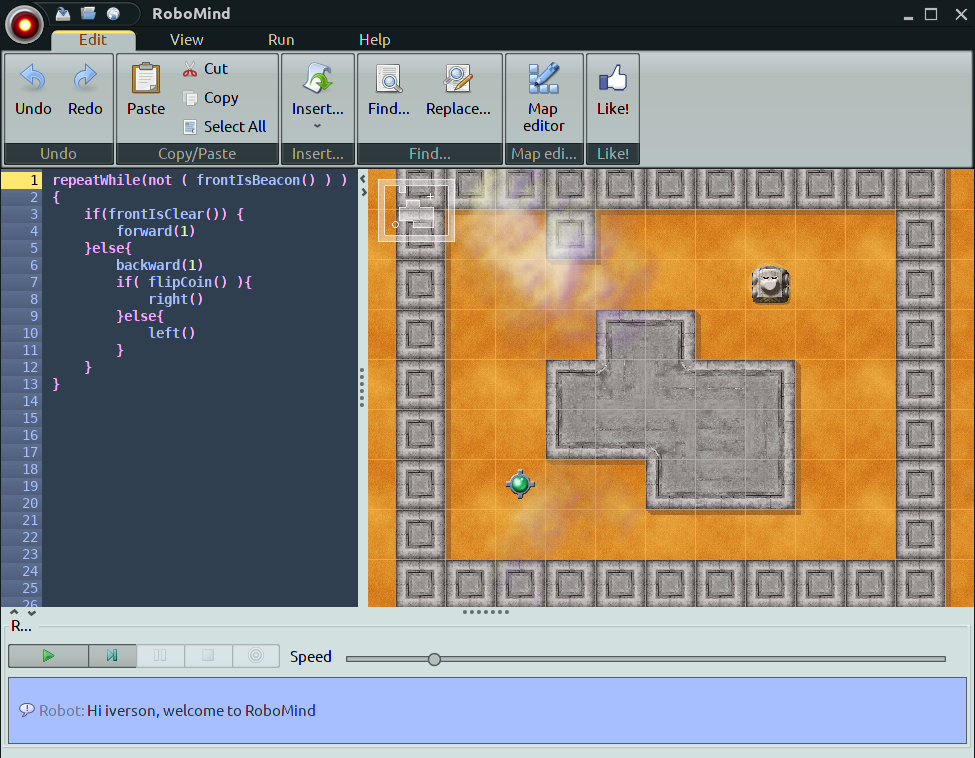
\includegraphics[height=10cm]{figuras/robomind_ide3.png}
\fonte{O autor}
\label{fig:robomind}
\end{figure}

\subsection{Linguagem ROBO}

É importante saber que a linguagem ROBO possui algumas características que a difere das linguagens de programação comuns. Abaixo estão listadas algumas das principais características de ROBO:

\begin{itemize}
    \item Funções booleanas predefinidas para detecção de obstáculos ou objetos ao redor do robô, por exemplo \textit{frontIsObstacle}, para verificar se há obstáculo na frente do robô ou \textit{frontIsClear}, para verificar se a frente do robô está livre de quaisquer objetos.
    \item Funções predefinidas para a movimentação do robô, como por exemplo \textit{forward(n)}, para movimentar para frente ou \textit{backward(n)}, para movimentar para trás.
    \item Definição de variáveis globais.
    \item Definição de procedimentos parametrizados e não parametrizados.
    \item Estruturas condicionais e de repetição, como por exemplo, \textit{if-else}, \textit{repeat(n)}, \textit{repeatWhile}
    \item Expressões aritméticas com valores inteiros.
\end{itemize}

\section{Métodos Formais}

No momento presente, o crescimento e a complexidade dos sistemas de software possibilita que falhas sejam empregadas durante o desenvolvimento, o que pode acarretar em prejuízos financeiros, despercício de tempo e, em sistemas críticos, perdas muitas vezes irreparáveis \cite{Clarke:1996}. Por essa razão, estudiosos da Engenharia de Software vêm propondo técnicas para auxiliar durante o processo de desenvolvimento, objetivando a construção de sistemas confiáveis para as mais diversas finalidades , como resultado, surgiram os métodos formais \cite{rui_silva}. Os métodos formais são baseados em principios matemáticos construídos a partir de linguagens formais. Por meio de técnicas e ferramentas para especificação de sistemas, os métodos formais são considerados um dos mais efetivos e rigorosos meios para a verificação de propriedades de sistemas, de modo a garantir que comportamentos indesejáveis não venham acontencer \cite{bhatt}.

A especificação formal é composta pela descrição de um sistema e suas propriedades em uma linguagem formal. Essa especificação formal deve ser sematicamente equivalente a modelagem original do sistema, só assim é possível garantir uma verificação consistente \cite{gannon}. A verificação formal utiliza a especificação para provar a descrição formal do sistema levando em consideração suas propriedades \cite{rui_silva}. Ou seja, é possível explorar os estados de um sistema considerando um conjunto de entradas e saídas, afirmando, assim, a corretude do sistema em relação às suas propriedades.

A verificação formal tem sido gradualmente aceita como um importante passo para a modelagem de sistemas críticos. O Verificador de Modelos (\textit{Model Checking}, em inglês) é uma das mais usadas dentre os métodos de verificação formal principalmente em sistemas concorrentes \cite{ZHAO2014}. Como estes verificadores proveem técnicas automáticas, sua utilização se torna muito efetiva para sistemas dessa finalidade.

\subsection{Verificação de Modelos}

Apesar de pouco utilizada no contexto educacional, a verificação automática de programas pode ser utilizada para obter \textit{feedback} automático sobre o funcionamento dos programas. Na literatura de métodos formais, existem duas principais técnicas de verificação, a Verificação de Modelos (\textit{Model Checking}) e a Verificação Dedutiva (\textit{Deductive Verification}). 

A técnica Verificação de Modelos é uma coleção de métodos para a verificação formal automatizada de sistemas concorrentes.  Consiste em utilizar como entradas para uma ferramenta de verificação de modelo (\textit{Model Checker}) um modelo do sistema, que pode ser expressado usando álgebra de processos ou até notação UML (\textit{Unified Modeling Language}), como também a especificação das propriedades que o sistema deve satisfazer \cite{FEIGN}. A Verificação de Modelos automaticamente analisa exaustivamente que a especificação de um sistema satifaz as propriedades definidas. Essa análise pode ser por meio de Lógica Temporal Linear (\textit{Linear Temporal Logic} - LTL) ou Lógica de Árvore de Computação (\textit{Computation Tree Logic} - CTL) \cite{ZHAO2014}. Como saída da verificação automática, temos o resultado positivo, se as propriedades são satisfeitas pelo modelo, ou resultado negativo, se as propriedades não são satisfeitas. Quando o resultado é negativo, o verificador de modelos mostra um cenário de execução onde o sistema não satisfaz alguma das propriedades, isso é chamado de contraexemplo. Uma desvantagem da Verificação de Modelos é que a técnica só consegue analisar sistemas com número finito e relativamente pequeno de estados. 

A técnica Verificação Dedutiva, diferentemente da anterior, é manual e requer maior conhecimento e experiência do usuário, entretanto, considera todos os estados possíveis do sistema, mesmo que sejam infinitos \cite{FEIGN}. Como neste trabalho estamos propondo a automatização da verificação, a técnica Verificação de Modelos é adotada como base para a verificação dos programas.

\subsection{Linguagem CSP}
\textit{Communicatting Sequential Processes} (CSP) é uma linguagem de álgebra de processos com o objetivo a especificação sistemas para ajudar na compreensão de sistemas concorrentes e distribuídos \cite{Cleaveland2018}. Essa linguagem é composta por processos e eventos que são utilizados para a especificação de um sistema, onde eventos são uma abstração para ocorrência dos fatos como, por exemplo, os comandos de movimentação do robô, e os processos definem a ordem de ocorrência dos eventos \cite{Roscoe2010}.

Foi em CSP que as funções do ambiente RoboMind foram modeladas por \cite{nogueira}, ou seja, se um programa ROBO e o mapa forem reescritos em CSP e executados em conjunto com esse modelo é possível executar os mesmos passos da simulação no ambiente RoboMind na especificação formal.

Existem várias ferramentas que podem ser utilizadas para a verificação de especificações escritas em CSP, as mais conhecidas são FDR\footnote[3]{https://www.cs.ox.ac.uk/projects/fdr/}, ProB\footnote[4]{https://www3.hhu.de/stups/prob} e PAT\footnote[5]{http://pat.comp.nus.edu.sg/}. Destas, a ferramenta FDR (\textit{Failures Divergence Refinement}) é a mais madura e utilizada; sua versão atual é FDR4 \cite{Gibson}. Por este motivo, este trabalho adota FDR4 como verificador de modelos.

\subsection{Verificador de Modelos FDR}

O verificador de modelos FDR, como citado, é o verificador de refinamento mais difundido para a álgebra de processo CSP. Este verificador utiliza a lista de processos CSP da especificação, e é capaz de verificar se os processos refinam uns aos outros de acordo com os modelos disponíveis na ferramenta: contraexemplo \textit{traces}; falhas (\textit{failures}); e falhas modelos de divergências (\textit{failures-divergences-models}). Além disso, é capaz de verificar outras propriedades: se o modelo está livre de \textit{deadlock} (\textit{deadlock-free}); se está livre de \textit{livelock} (\textit{livelock-free}) e verificação de determinismo \cite{Gibson}.

Na Figura \ref{fig:assertion} tem um exemplo de verificação de uma propriedade em FDR. As propriedades são chamadas de \textit{Assertions}, onde logo abaixo tem a lista de propriedades definidas em uma especificação CSP. Nesse caso, a propriedade analisada é se \texttt{PROGRAM} possui \textit{deadlock}, dada por \texttt{:[deadlock free [F]]}. Como o resultado falhou (\textit{Failed}), então o \texttt{PROGRAM} termina sua execução.

\begin{figure}[h]
\centering
\caption{Exemplo de verificação da propriedade \textit{deadlock-free}}
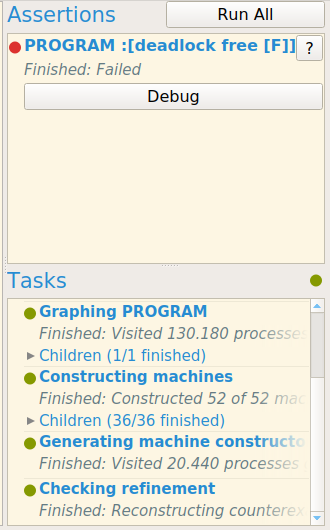
\includegraphics[height=10cm]{figuras/assertion.png}
\fonte{O autor}
\label{fig:assertion}
\end{figure}

A ferramenta FDR ainda provê um \textit{feedback} visual da especificação dos sistemas. Está disposto na Figura \ref{fig:graph} parte da máquina de estados de um processo chamado \texttt{COMMANDS}. Cada estado representa um possível evento que possa ocorrer e em cada um deles há os possíveis outros estados que são acessíveis pelos os mesmos. Por exemplo, o evento inicial \texttt{right} pode dar origem a outros quatro eventos: \texttt{get.ORIENTATION.0}, \texttt{get.ORIENTATION.1}, \texttt{get.ORIENTATION.2} ou \texttt{get.ORIENTATION.3}.

Diante disso, podemos afirmar que FDR de fato é uma ferramenta poderosa para esses tipos de verificações em cima de sistemas modelados em CSP, a fim de explorar possibilidades que o próprio sistema sozinho não fornece. O verificador de modelos FDR ainda possui uma API (\textit{Application Programming Interface}) propiciando a projetação de sistemas integrados à ferramenta.

\begin{figure}[h]
\centering
\caption{Máquina de estados de um processo CSP}
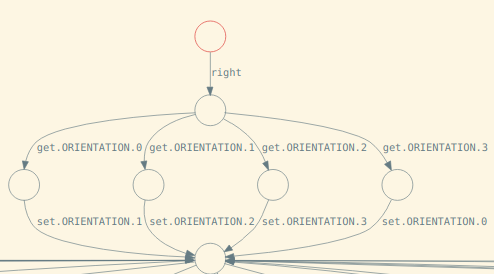
\includegraphics[height=7cm]{figuras/graph.png}
\fonte{O autor}
\label{fig:graph}
\end{figure}

\section{Processo de Compilação}

\subsection{Linguagem de Domínio Específico - DSL}
Uma Linguagem de Domínio Específico (\textit{Domain-Specific Language} - DSL) como o próprio já diz é uma linguagem que possui um propósito bem definido, diferente das linguagens de propósito geral, como por exemplo, Java ou C. A criação de DSLs tem como característica a possibilidade de expressar soluções para problemas de modo mais claro que as linguagens de próposito geral \cite{fowler}.

A criação de um compilador para uma DSL depende do tipo da DSL. Geralmente para uma DSL interna, isto é, uma linguagem que é executada em cima de um compilador de uma linguagem de propósito geral, é necessário que a linguagem tenha o compilador modificado. Já para as DSLs externas, um novo compilador ou interpretador deve ser implementando \cite{schimitt}.

Sabendo disso, a linguagem ROBO é um tipo de DSL que tem como finalidade a criação de programas para a simulação de robôs em um ambiente virtual. para criar um compilador para esta linguagem é necessário um mecanismo que ajude nesse processo, e uma d

\section{Plataforma \textit{Spoofax}}
\textit{Spoofax}\footnote[6]{http://www.metaborg.org/} é uma platafoma para desenvolvimento textual de liguagens de programação. Esta plataforma permite o desenvolvimento através de um ambiente interativo usando metalinguagens (\textit{meta-languages)} para definição de linguagem declarativa de alto nível. Além disso, possui geradores de código que produzem analisadores (\textit{parses}), checagem de tipo, compiladores, interpretadores e outras ferramentas. A vantagem de usar \textit{Spoofax} é o foco na essência da definição da linguagem, ignorando detalhes irrelevantes da implementação \cite{KatsSpoofax}.

Um projeto em \textit{Spoofax} possui uma arquitetura muito bem estruturada, seguindo alguns princípios. Primeiro, separação de interesses, por exemplo, separa definição de sintaxe da definição da semântica estática. Segundo, não repete aspectos da linguagem em diferentes implementções, objetivando a geração de diferentes artefatos a partir de um único código. Por último, a definição de linguagem declarativa ocorre de modo independente, onde cada tipo de implementação possui sua própria linguagem correspondente. Por exemplo, para definição de sintaxe utiliza o formalismo SDF3, já para a parte de transformação, utiliza-se a linguagem \textit{Stratego} \cite{KatsSpoofax}. \textit{Spoofax} ainda provê outras metalinguagens, como por exemplo NaBL2, utilizada para a checagem semâtica da linguagem, o que inclui checagem de nomes e análise de tipos. 

Para o escopo desse projeto, apenas utilizou-se SDF3 e \textit{Stratego}, tendo em vista que a checagem de nomes e tipos não seria uma prioridade neste momento, uma vez que os programas ROBO são executados previamente no RoboMind que possui esse tipo de análise.

Assim como o verificador de modelos FDR, a plataforma \textit{Spoofax} dispõe de uma API que pode ser utilizada para diferentes objetivos, como por exemplo, o desenvolvimento de ferramentas integradas a um compilador gerado pela plataforma.

\subsection{Definição Sintática}

A definição sintática com \textit{Spoofax} ocorre através da metalinguagem SDF3, esta é um formalismo que propicia a definição da sintaxe para linguagens de programação e DSLs. Na Figura \ref{fig:parsing} é mostrado o fluxograma de como ocorre a definição sintática com essa plataforma, desde a definição da gramática até a geração da árvore sintática. O primeiro passo é a definição dos módulos em SDF3, onde ocorre toda a geração da gramática da linguagem. Como saída dos módulos normalizados em SDF3, é gerada uma tabela de análise (\textit{Parse Table}) que é utilizado como entrada no \textit{Scannerless Generalized LR} (SGLR), responsável por produzir a Árvore de Sintaxe Abstrata (\textit{Abstract Syntax Tree} - AST). Após a geração de uma AST, o SDF3 conta com uma mecanismo que remove todas as ambiguidades, gerando uma única AST (\textit{Parse Tree}) de um programa em uma linguagem específica (\textit{Source Program}). 

\begin{figure}[h]
\centering
\caption{Processo de definição sintática do Spoofax}
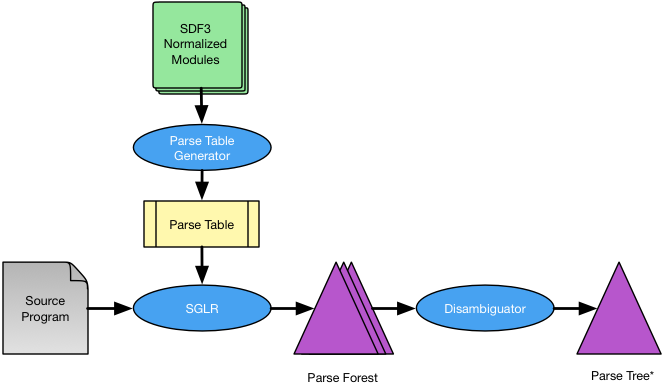
\includegraphics[height=7cm]{figuras/parsing.png}
\fonte{\cite{metaborg}}
\label{fig:parsing}
\end{figure}

A Figura \ref{fig:sdf} mostra como é a estrutura de um ambiente de programação utilizando essa metalinguagem. Na parte mais a esquerda da figura tem um exemplo (\textit{Example.sdf3}) onde há a definição sintática de uma linguagem. Esse exemplo é um módulo (\texttt{module}) que é constituído por seções. Nos três quadros da direita, estão dispostos três arquivos. No quadrante de cima mostra como é a interação durante uma codifição de um programa na linguagem definida, mostrando sugestões da gramática. No quadro do meio, mostra um exemplo formatado de código aceito pela gramática. E no último quadro (\textit{Example.aterm}) é mostrado a árvore sitática do programa \textit{Example.tes}.

\begin{figure}[h]
\centering
\caption{Definição sintática com SDF3}
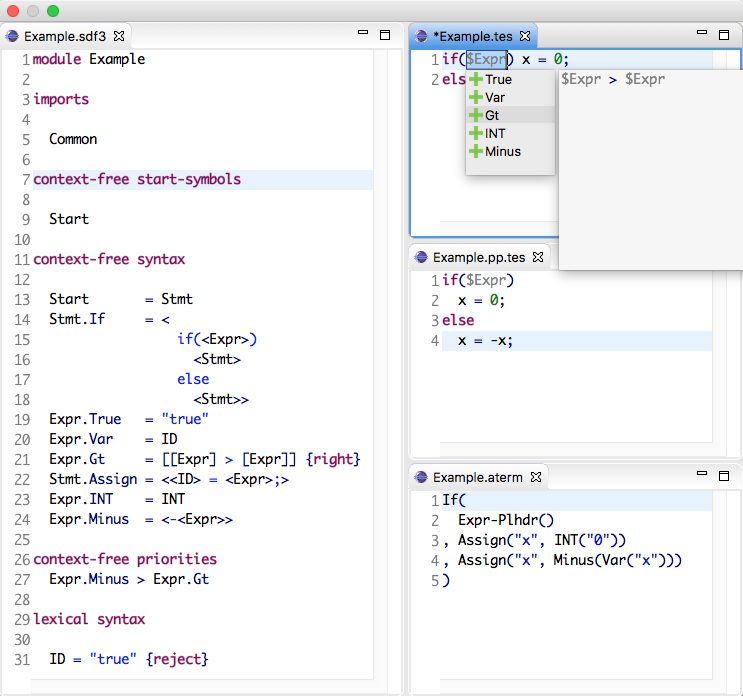
\includegraphics[height=10cm]{figuras/sdf3-spoofax.png}
\fonte{\cite{metaborg}}
\label{fig:sdf}
\end{figure}

Todas essas seções da figura citada anteriormente são importantes para a definição final da gramática de uma linguagem. A seção \textit{} \texttt{context-free start-symbols} indica os símbolos iniciais quando ocorre uma análise dos termos. A seção \texttt{context-free syntax} descreve em alto nível a estrutura sintática das sentenças em uma linguagem, contendo uma lista de produções. A seção \texttt{context-free priorities} é utilizado para remover ambiguidades através da definição de prioridades entre as produções. Por último, a seção \texttt{lexical syntax} descreve a parte léxica da linguagem, ou seja, como cada produção deve ser representada e também a definição de palavras reservadas da linguagem.

A definição sintática com \textit{Spoofax}, mais especificamente usando a metalinguagem SDF3, como visto, ocorre de modo alto nível, facilitando todo esse processo. Como produto disso, temos uma árvore sintática não ambígua que é essencial para a etapa seguinte do processo de compilação, a geração de código. A transformação ocorre através da metalinguagem \textit{Stratego} que será explicada a seguir.

\subsection{Transformação}
